\documentclass[aspectratio=169]{beamer}
% Shared preamble for ml/ slide decks.
% Each lecture .tex starts with:
%   \documentclass[aspectratio=169]{beamer}
%   % Shared preamble for ml/ slide decks.
% Each lecture .tex starts with:
%   \documentclass[aspectratio=169]{beamer}
%   % Shared preamble for ml/ slide decks.
% Each lecture .tex starts with:
%   \documentclass[aspectratio=169]{beamer}
%   \input{../preamble}
% Compile from inside the chapter folder so \input{../preamble} resolves.

\usetheme{default}
\usecolortheme{dove}

\setbeamertemplate{navigation symbols}{}
\setbeamertemplate{footline}{%
  \hfill{\large\insertframenumber\,/\,\inserttotalframenumber}\hspace{0.8em}\vspace{0.5em}%
}

% Project palette (existing, kept for backwards compatibility with deferred/*)
\definecolor{popblue}{RGB}{52, 101, 164}
\definecolor{sampred}{RGB}{204, 0, 0}
\definecolor{paramgreen}{RGB}{0, 140, 70}
\definecolor{warnred}{RGB}{180, 40, 40}
\definecolor{orange1}{RGB}{220, 120, 0}
\definecolor{violet1}{RGB}{120, 50, 160}
\definecolor{lightbg}{RGB}{245, 245, 250}

% Armenian flag palette (use these for any 3-color highlight; per CLAUDE.md).
% "Nice versions": slightly de-saturated from the official spec for slide use,
% so they don't burn out under projector colors. Originals kept as *_pure.
\definecolor{armred}{RGB}{200, 30, 40}      % nice red (official #D90012 muted)
\definecolor{armblue}{RGB}{30, 70, 160}     % nice blue (official #0033A0 muted)
\definecolor{armorange}{RGB}{230, 160, 30}  % nice orange (official #F2A800 muted)
\definecolor{armred_pure}{HTML}{D90012}     % official Armenian flag red
\definecolor{armblue_pure}{HTML}{0033A0}    % official Armenian flag blue
\definecolor{armorange_pure}{HTML}{F2A800}  % official Armenian flag orange

\setbeamercolor{frametitle}{fg=popblue}
\setbeamercolor{title}{fg=popblue}

\usepackage{pgfplots}
\usepackage{tikz}
\usetikzlibrary{shapes, arrows.meta, positioning, calc, decorations.pathreplacing, patterns, matrix}
\pgfplotsset{compat=1.18}
\usepackage{amsmath, amssymb, amsfonts}
\usepackage{bm}
\usepackage{dsfont}
\usepackage{array}
\usepackage{pifont}
\usepackage{colortbl}
\usepackage{fontenc}

% Callout boxes. Purely additive - existing decks are unaffected.
% Usage: \begin{tcolorbox}[colback=armblue!8, colframe=armblue, boxrule=0.6pt, arc=2pt,
%                          title=\textbf{Key idea}] ... \end{tcolorbox}
% Palette convention (ml/SLIDE_STYLE.md): armblue=key idea, armred=trap/warning,
% paramgreen=takeaway or "Next", armorange=watch-out.
\usepackage[most]{tcolorbox}

% Cleaner table rules (\toprule, \midrule, \bottomrule). Also purely additive.
\usepackage{booktabs}

% \cancel{...} for struck-through terms in derivations (added 2026-08-11 for the
% importance-sampling frame in ch11_rl, where the dynamics cancel). Purely additive.
\usepackage{cancel}

% Minimal ML notation macros (subset of slds-lmu latex-math/basic-ml.tex).
% Kept here so we don't have to inline-expand every \thetav, \xv, etc.
% when porting upstream slides.
\newcommand{\R}{\mathds{R}}
\newcommand{\N}{\mathds{N}}
\newcommand{\E}{\mathds{E}}
\newcommand{\Xspace}{\mathcal{X}}
\newcommand{\Yspace}{\mathcal{Y}}
\newcommand{\Hspace}{\mathcal{H}}
\newcommand{\D}{\mathcal{D}}
\newcommand{\Dtrain}{\mathcal{D}_{\text{train}}}
\newcommand{\Dtest}{\mathcal{D}_{\text{test}}}
\newcommand{\xv}{\mathbf{x}}
\newcommand{\yv}{\mathbf{y}}
\newcommand{\Xmat}{\mathbf{X}}
\newcommand{\id}{\mathbf{I}}
\newcommand{\thetav}{\bm{\theta}}
\newcommand{\thetah}{\hat{\bm{\theta}}}
\newcommand{\lamv}{\bm{\lambda}}
\newcommand{\fx}{f(\xv)}
\newcommand{\fxt}{f(\xv \,|\, \bm{\theta})}
\newcommand{\fxi}{f\!\left(\xv^{(i)}\right)}
\newcommand{\fh}{\hat{f}}
\newcommand{\fxh}{\hat{f}(\xv)}
\newcommand{\yh}{\hat{y}}
\newcommand{\yih}{\hat{y}^{(i)}}
% \xi clashes with the Greek letter \xi; write \xv^{(i)} inline instead.
\newcommand{\yi}[1][i]{y^{(#1)}}
\newcommand{\xyi}[1][i]{\left(\xv^{(#1)},\, y^{(#1)}\right)}
\newcommand{\thx}{\bm{\theta}^\top \xv}
\newcommand{\sumin}{\sum_{i=1}^{n}}
\newcommand{\sumjp}{\sum_{j=1}^{p}}
\newcommand{\Lxy}{L\!\left(y, \fx\right)}
\newcommand{\Lxyi}{L\!\left(\yi, \fxi\right)}
\newcommand{\risk}{\mathcal{R}}
\newcommand{\riske}{\mathcal{R}_{\text{emp}}}
\newcommand{\risket}{\mathcal{R}_{\text{emp}}(\bm{\theta})}
\newcommand{\riskt}{\mathcal{R}(\bm{\theta})}
\newcommand{\riskr}{\mathcal{R}_{\text{reg}}}
\newcommand{\argmin}{\mathop{\mathrm{arg\,min}}}
\newcommand{\argmax}{\mathop{\mathrm{arg\,max}}}
\newcommand{\eps}{\varepsilon}

% Compile from inside the chapter folder so % Shared preamble for ml/ slide decks.
% Each lecture .tex starts with:
%   \documentclass[aspectratio=169]{beamer}
%   \input{../preamble}
% Compile from inside the chapter folder so \input{../preamble} resolves.

\usetheme{default}
\usecolortheme{dove}

\setbeamertemplate{navigation symbols}{}
\setbeamertemplate{footline}{%
  \hfill{\large\insertframenumber\,/\,\inserttotalframenumber}\hspace{0.8em}\vspace{0.5em}%
}

% Project palette (existing, kept for backwards compatibility with deferred/*)
\definecolor{popblue}{RGB}{52, 101, 164}
\definecolor{sampred}{RGB}{204, 0, 0}
\definecolor{paramgreen}{RGB}{0, 140, 70}
\definecolor{warnred}{RGB}{180, 40, 40}
\definecolor{orange1}{RGB}{220, 120, 0}
\definecolor{violet1}{RGB}{120, 50, 160}
\definecolor{lightbg}{RGB}{245, 245, 250}

% Armenian flag palette (use these for any 3-color highlight; per CLAUDE.md).
% "Nice versions": slightly de-saturated from the official spec for slide use,
% so they don't burn out under projector colors. Originals kept as *_pure.
\definecolor{armred}{RGB}{200, 30, 40}      % nice red (official #D90012 muted)
\definecolor{armblue}{RGB}{30, 70, 160}     % nice blue (official #0033A0 muted)
\definecolor{armorange}{RGB}{230, 160, 30}  % nice orange (official #F2A800 muted)
\definecolor{armred_pure}{HTML}{D90012}     % official Armenian flag red
\definecolor{armblue_pure}{HTML}{0033A0}    % official Armenian flag blue
\definecolor{armorange_pure}{HTML}{F2A800}  % official Armenian flag orange

\setbeamercolor{frametitle}{fg=popblue}
\setbeamercolor{title}{fg=popblue}

\usepackage{pgfplots}
\usepackage{tikz}
\usetikzlibrary{shapes, arrows.meta, positioning, calc, decorations.pathreplacing, patterns, matrix}
\pgfplotsset{compat=1.18}
\usepackage{amsmath, amssymb, amsfonts}
\usepackage{bm}
\usepackage{dsfont}
\usepackage{array}
\usepackage{pifont}
\usepackage{colortbl}
\usepackage{fontenc}

% Callout boxes. Purely additive - existing decks are unaffected.
% Usage: \begin{tcolorbox}[colback=armblue!8, colframe=armblue, boxrule=0.6pt, arc=2pt,
%                          title=\textbf{Key idea}] ... \end{tcolorbox}
% Palette convention (ml/SLIDE_STYLE.md): armblue=key idea, armred=trap/warning,
% paramgreen=takeaway or "Next", armorange=watch-out.
\usepackage[most]{tcolorbox}

% Cleaner table rules (\toprule, \midrule, \bottomrule). Also purely additive.
\usepackage{booktabs}

% \cancel{...} for struck-through terms in derivations (added 2026-08-11 for the
% importance-sampling frame in ch11_rl, where the dynamics cancel). Purely additive.
\usepackage{cancel}

% Minimal ML notation macros (subset of slds-lmu latex-math/basic-ml.tex).
% Kept here so we don't have to inline-expand every \thetav, \xv, etc.
% when porting upstream slides.
\newcommand{\R}{\mathds{R}}
\newcommand{\N}{\mathds{N}}
\newcommand{\E}{\mathds{E}}
\newcommand{\Xspace}{\mathcal{X}}
\newcommand{\Yspace}{\mathcal{Y}}
\newcommand{\Hspace}{\mathcal{H}}
\newcommand{\D}{\mathcal{D}}
\newcommand{\Dtrain}{\mathcal{D}_{\text{train}}}
\newcommand{\Dtest}{\mathcal{D}_{\text{test}}}
\newcommand{\xv}{\mathbf{x}}
\newcommand{\yv}{\mathbf{y}}
\newcommand{\Xmat}{\mathbf{X}}
\newcommand{\id}{\mathbf{I}}
\newcommand{\thetav}{\bm{\theta}}
\newcommand{\thetah}{\hat{\bm{\theta}}}
\newcommand{\lamv}{\bm{\lambda}}
\newcommand{\fx}{f(\xv)}
\newcommand{\fxt}{f(\xv \,|\, \bm{\theta})}
\newcommand{\fxi}{f\!\left(\xv^{(i)}\right)}
\newcommand{\fh}{\hat{f}}
\newcommand{\fxh}{\hat{f}(\xv)}
\newcommand{\yh}{\hat{y}}
\newcommand{\yih}{\hat{y}^{(i)}}
% \xi clashes with the Greek letter \xi; write \xv^{(i)} inline instead.
\newcommand{\yi}[1][i]{y^{(#1)}}
\newcommand{\xyi}[1][i]{\left(\xv^{(#1)},\, y^{(#1)}\right)}
\newcommand{\thx}{\bm{\theta}^\top \xv}
\newcommand{\sumin}{\sum_{i=1}^{n}}
\newcommand{\sumjp}{\sum_{j=1}^{p}}
\newcommand{\Lxy}{L\!\left(y, \fx\right)}
\newcommand{\Lxyi}{L\!\left(\yi, \fxi\right)}
\newcommand{\risk}{\mathcal{R}}
\newcommand{\riske}{\mathcal{R}_{\text{emp}}}
\newcommand{\risket}{\mathcal{R}_{\text{emp}}(\bm{\theta})}
\newcommand{\riskt}{\mathcal{R}(\bm{\theta})}
\newcommand{\riskr}{\mathcal{R}_{\text{reg}}}
\newcommand{\argmin}{\mathop{\mathrm{arg\,min}}}
\newcommand{\argmax}{\mathop{\mathrm{arg\,max}}}
\newcommand{\eps}{\varepsilon}
 resolves.

\usetheme{default}
\usecolortheme{dove}

\setbeamertemplate{navigation symbols}{}
\setbeamertemplate{footline}{%
  \hfill{\large\insertframenumber\,/\,\inserttotalframenumber}\hspace{0.8em}\vspace{0.5em}%
}

% Project palette (existing, kept for backwards compatibility with deferred/*)
\definecolor{popblue}{RGB}{52, 101, 164}
\definecolor{sampred}{RGB}{204, 0, 0}
\definecolor{paramgreen}{RGB}{0, 140, 70}
\definecolor{warnred}{RGB}{180, 40, 40}
\definecolor{orange1}{RGB}{220, 120, 0}
\definecolor{violet1}{RGB}{120, 50, 160}
\definecolor{lightbg}{RGB}{245, 245, 250}

% Armenian flag palette (use these for any 3-color highlight; per CLAUDE.md).
% "Nice versions": slightly de-saturated from the official spec for slide use,
% so they don't burn out under projector colors. Originals kept as *_pure.
\definecolor{armred}{RGB}{200, 30, 40}      % nice red (official #D90012 muted)
\definecolor{armblue}{RGB}{30, 70, 160}     % nice blue (official #0033A0 muted)
\definecolor{armorange}{RGB}{230, 160, 30}  % nice orange (official #F2A800 muted)
\definecolor{armred_pure}{HTML}{D90012}     % official Armenian flag red
\definecolor{armblue_pure}{HTML}{0033A0}    % official Armenian flag blue
\definecolor{armorange_pure}{HTML}{F2A800}  % official Armenian flag orange

\setbeamercolor{frametitle}{fg=popblue}
\setbeamercolor{title}{fg=popblue}

\usepackage{pgfplots}
\usepackage{tikz}
\usetikzlibrary{shapes, arrows.meta, positioning, calc, decorations.pathreplacing, patterns, matrix}
\pgfplotsset{compat=1.18}
\usepackage{amsmath, amssymb, amsfonts}
\usepackage{bm}
\usepackage{dsfont}
\usepackage{array}
\usepackage{pifont}
\usepackage{colortbl}
\usepackage{fontenc}

% Callout boxes. Purely additive - existing decks are unaffected.
% Usage: \begin{tcolorbox}[colback=armblue!8, colframe=armblue, boxrule=0.6pt, arc=2pt,
%                          title=\textbf{Key idea}] ... \end{tcolorbox}
% Palette convention (ml/SLIDE_STYLE.md): armblue=key idea, armred=trap/warning,
% paramgreen=takeaway or "Next", armorange=watch-out.
\usepackage[most]{tcolorbox}

% Cleaner table rules (\toprule, \midrule, \bottomrule). Also purely additive.
\usepackage{booktabs}

% \cancel{...} for struck-through terms in derivations (added 2026-08-11 for the
% importance-sampling frame in ch11_rl, where the dynamics cancel). Purely additive.
\usepackage{cancel}

% Minimal ML notation macros (subset of slds-lmu latex-math/basic-ml.tex).
% Kept here so we don't have to inline-expand every \thetav, \xv, etc.
% when porting upstream slides.
\newcommand{\R}{\mathds{R}}
\newcommand{\N}{\mathds{N}}
\newcommand{\E}{\mathds{E}}
\newcommand{\Xspace}{\mathcal{X}}
\newcommand{\Yspace}{\mathcal{Y}}
\newcommand{\Hspace}{\mathcal{H}}
\newcommand{\D}{\mathcal{D}}
\newcommand{\Dtrain}{\mathcal{D}_{\text{train}}}
\newcommand{\Dtest}{\mathcal{D}_{\text{test}}}
\newcommand{\xv}{\mathbf{x}}
\newcommand{\yv}{\mathbf{y}}
\newcommand{\Xmat}{\mathbf{X}}
\newcommand{\id}{\mathbf{I}}
\newcommand{\thetav}{\bm{\theta}}
\newcommand{\thetah}{\hat{\bm{\theta}}}
\newcommand{\lamv}{\bm{\lambda}}
\newcommand{\fx}{f(\xv)}
\newcommand{\fxt}{f(\xv \,|\, \bm{\theta})}
\newcommand{\fxi}{f\!\left(\xv^{(i)}\right)}
\newcommand{\fh}{\hat{f}}
\newcommand{\fxh}{\hat{f}(\xv)}
\newcommand{\yh}{\hat{y}}
\newcommand{\yih}{\hat{y}^{(i)}}
% \xi clashes with the Greek letter \xi; write \xv^{(i)} inline instead.
\newcommand{\yi}[1][i]{y^{(#1)}}
\newcommand{\xyi}[1][i]{\left(\xv^{(#1)},\, y^{(#1)}\right)}
\newcommand{\thx}{\bm{\theta}^\top \xv}
\newcommand{\sumin}{\sum_{i=1}^{n}}
\newcommand{\sumjp}{\sum_{j=1}^{p}}
\newcommand{\Lxy}{L\!\left(y, \fx\right)}
\newcommand{\Lxyi}{L\!\left(\yi, \fxi\right)}
\newcommand{\risk}{\mathcal{R}}
\newcommand{\riske}{\mathcal{R}_{\text{emp}}}
\newcommand{\risket}{\mathcal{R}_{\text{emp}}(\bm{\theta})}
\newcommand{\riskt}{\mathcal{R}(\bm{\theta})}
\newcommand{\riskr}{\mathcal{R}_{\text{reg}}}
\newcommand{\argmin}{\mathop{\mathrm{arg\,min}}}
\newcommand{\argmax}{\mathop{\mathrm{arg\,max}}}
\newcommand{\eps}{\varepsilon}

% Compile from inside the chapter folder so % Shared preamble for ml/ slide decks.
% Each lecture .tex starts with:
%   \documentclass[aspectratio=169]{beamer}
%   % Shared preamble for ml/ slide decks.
% Each lecture .tex starts with:
%   \documentclass[aspectratio=169]{beamer}
%   \input{../preamble}
% Compile from inside the chapter folder so \input{../preamble} resolves.

\usetheme{default}
\usecolortheme{dove}

\setbeamertemplate{navigation symbols}{}
\setbeamertemplate{footline}{%
  \hfill{\large\insertframenumber\,/\,\inserttotalframenumber}\hspace{0.8em}\vspace{0.5em}%
}

% Project palette (existing, kept for backwards compatibility with deferred/*)
\definecolor{popblue}{RGB}{52, 101, 164}
\definecolor{sampred}{RGB}{204, 0, 0}
\definecolor{paramgreen}{RGB}{0, 140, 70}
\definecolor{warnred}{RGB}{180, 40, 40}
\definecolor{orange1}{RGB}{220, 120, 0}
\definecolor{violet1}{RGB}{120, 50, 160}
\definecolor{lightbg}{RGB}{245, 245, 250}

% Armenian flag palette (use these for any 3-color highlight; per CLAUDE.md).
% "Nice versions": slightly de-saturated from the official spec for slide use,
% so they don't burn out under projector colors. Originals kept as *_pure.
\definecolor{armred}{RGB}{200, 30, 40}      % nice red (official #D90012 muted)
\definecolor{armblue}{RGB}{30, 70, 160}     % nice blue (official #0033A0 muted)
\definecolor{armorange}{RGB}{230, 160, 30}  % nice orange (official #F2A800 muted)
\definecolor{armred_pure}{HTML}{D90012}     % official Armenian flag red
\definecolor{armblue_pure}{HTML}{0033A0}    % official Armenian flag blue
\definecolor{armorange_pure}{HTML}{F2A800}  % official Armenian flag orange

\setbeamercolor{frametitle}{fg=popblue}
\setbeamercolor{title}{fg=popblue}

\usepackage{pgfplots}
\usepackage{tikz}
\usetikzlibrary{shapes, arrows.meta, positioning, calc, decorations.pathreplacing, patterns, matrix}
\pgfplotsset{compat=1.18}
\usepackage{amsmath, amssymb, amsfonts}
\usepackage{bm}
\usepackage{dsfont}
\usepackage{array}
\usepackage{pifont}
\usepackage{colortbl}
\usepackage{fontenc}

% Callout boxes. Purely additive - existing decks are unaffected.
% Usage: \begin{tcolorbox}[colback=armblue!8, colframe=armblue, boxrule=0.6pt, arc=2pt,
%                          title=\textbf{Key idea}] ... \end{tcolorbox}
% Palette convention (ml/SLIDE_STYLE.md): armblue=key idea, armred=trap/warning,
% paramgreen=takeaway or "Next", armorange=watch-out.
\usepackage[most]{tcolorbox}

% Cleaner table rules (\toprule, \midrule, \bottomrule). Also purely additive.
\usepackage{booktabs}

% \cancel{...} for struck-through terms in derivations (added 2026-08-11 for the
% importance-sampling frame in ch11_rl, where the dynamics cancel). Purely additive.
\usepackage{cancel}

% Minimal ML notation macros (subset of slds-lmu latex-math/basic-ml.tex).
% Kept here so we don't have to inline-expand every \thetav, \xv, etc.
% when porting upstream slides.
\newcommand{\R}{\mathds{R}}
\newcommand{\N}{\mathds{N}}
\newcommand{\E}{\mathds{E}}
\newcommand{\Xspace}{\mathcal{X}}
\newcommand{\Yspace}{\mathcal{Y}}
\newcommand{\Hspace}{\mathcal{H}}
\newcommand{\D}{\mathcal{D}}
\newcommand{\Dtrain}{\mathcal{D}_{\text{train}}}
\newcommand{\Dtest}{\mathcal{D}_{\text{test}}}
\newcommand{\xv}{\mathbf{x}}
\newcommand{\yv}{\mathbf{y}}
\newcommand{\Xmat}{\mathbf{X}}
\newcommand{\id}{\mathbf{I}}
\newcommand{\thetav}{\bm{\theta}}
\newcommand{\thetah}{\hat{\bm{\theta}}}
\newcommand{\lamv}{\bm{\lambda}}
\newcommand{\fx}{f(\xv)}
\newcommand{\fxt}{f(\xv \,|\, \bm{\theta})}
\newcommand{\fxi}{f\!\left(\xv^{(i)}\right)}
\newcommand{\fh}{\hat{f}}
\newcommand{\fxh}{\hat{f}(\xv)}
\newcommand{\yh}{\hat{y}}
\newcommand{\yih}{\hat{y}^{(i)}}
% \xi clashes with the Greek letter \xi; write \xv^{(i)} inline instead.
\newcommand{\yi}[1][i]{y^{(#1)}}
\newcommand{\xyi}[1][i]{\left(\xv^{(#1)},\, y^{(#1)}\right)}
\newcommand{\thx}{\bm{\theta}^\top \xv}
\newcommand{\sumin}{\sum_{i=1}^{n}}
\newcommand{\sumjp}{\sum_{j=1}^{p}}
\newcommand{\Lxy}{L\!\left(y, \fx\right)}
\newcommand{\Lxyi}{L\!\left(\yi, \fxi\right)}
\newcommand{\risk}{\mathcal{R}}
\newcommand{\riske}{\mathcal{R}_{\text{emp}}}
\newcommand{\risket}{\mathcal{R}_{\text{emp}}(\bm{\theta})}
\newcommand{\riskt}{\mathcal{R}(\bm{\theta})}
\newcommand{\riskr}{\mathcal{R}_{\text{reg}}}
\newcommand{\argmin}{\mathop{\mathrm{arg\,min}}}
\newcommand{\argmax}{\mathop{\mathrm{arg\,max}}}
\newcommand{\eps}{\varepsilon}

% Compile from inside the chapter folder so % Shared preamble for ml/ slide decks.
% Each lecture .tex starts with:
%   \documentclass[aspectratio=169]{beamer}
%   \input{../preamble}
% Compile from inside the chapter folder so \input{../preamble} resolves.

\usetheme{default}
\usecolortheme{dove}

\setbeamertemplate{navigation symbols}{}
\setbeamertemplate{footline}{%
  \hfill{\large\insertframenumber\,/\,\inserttotalframenumber}\hspace{0.8em}\vspace{0.5em}%
}

% Project palette (existing, kept for backwards compatibility with deferred/*)
\definecolor{popblue}{RGB}{52, 101, 164}
\definecolor{sampred}{RGB}{204, 0, 0}
\definecolor{paramgreen}{RGB}{0, 140, 70}
\definecolor{warnred}{RGB}{180, 40, 40}
\definecolor{orange1}{RGB}{220, 120, 0}
\definecolor{violet1}{RGB}{120, 50, 160}
\definecolor{lightbg}{RGB}{245, 245, 250}

% Armenian flag palette (use these for any 3-color highlight; per CLAUDE.md).
% "Nice versions": slightly de-saturated from the official spec for slide use,
% so they don't burn out under projector colors. Originals kept as *_pure.
\definecolor{armred}{RGB}{200, 30, 40}      % nice red (official #D90012 muted)
\definecolor{armblue}{RGB}{30, 70, 160}     % nice blue (official #0033A0 muted)
\definecolor{armorange}{RGB}{230, 160, 30}  % nice orange (official #F2A800 muted)
\definecolor{armred_pure}{HTML}{D90012}     % official Armenian flag red
\definecolor{armblue_pure}{HTML}{0033A0}    % official Armenian flag blue
\definecolor{armorange_pure}{HTML}{F2A800}  % official Armenian flag orange

\setbeamercolor{frametitle}{fg=popblue}
\setbeamercolor{title}{fg=popblue}

\usepackage{pgfplots}
\usepackage{tikz}
\usetikzlibrary{shapes, arrows.meta, positioning, calc, decorations.pathreplacing, patterns, matrix}
\pgfplotsset{compat=1.18}
\usepackage{amsmath, amssymb, amsfonts}
\usepackage{bm}
\usepackage{dsfont}
\usepackage{array}
\usepackage{pifont}
\usepackage{colortbl}
\usepackage{fontenc}

% Callout boxes. Purely additive - existing decks are unaffected.
% Usage: \begin{tcolorbox}[colback=armblue!8, colframe=armblue, boxrule=0.6pt, arc=2pt,
%                          title=\textbf{Key idea}] ... \end{tcolorbox}
% Palette convention (ml/SLIDE_STYLE.md): armblue=key idea, armred=trap/warning,
% paramgreen=takeaway or "Next", armorange=watch-out.
\usepackage[most]{tcolorbox}

% Cleaner table rules (\toprule, \midrule, \bottomrule). Also purely additive.
\usepackage{booktabs}

% \cancel{...} for struck-through terms in derivations (added 2026-08-11 for the
% importance-sampling frame in ch11_rl, where the dynamics cancel). Purely additive.
\usepackage{cancel}

% Minimal ML notation macros (subset of slds-lmu latex-math/basic-ml.tex).
% Kept here so we don't have to inline-expand every \thetav, \xv, etc.
% when porting upstream slides.
\newcommand{\R}{\mathds{R}}
\newcommand{\N}{\mathds{N}}
\newcommand{\E}{\mathds{E}}
\newcommand{\Xspace}{\mathcal{X}}
\newcommand{\Yspace}{\mathcal{Y}}
\newcommand{\Hspace}{\mathcal{H}}
\newcommand{\D}{\mathcal{D}}
\newcommand{\Dtrain}{\mathcal{D}_{\text{train}}}
\newcommand{\Dtest}{\mathcal{D}_{\text{test}}}
\newcommand{\xv}{\mathbf{x}}
\newcommand{\yv}{\mathbf{y}}
\newcommand{\Xmat}{\mathbf{X}}
\newcommand{\id}{\mathbf{I}}
\newcommand{\thetav}{\bm{\theta}}
\newcommand{\thetah}{\hat{\bm{\theta}}}
\newcommand{\lamv}{\bm{\lambda}}
\newcommand{\fx}{f(\xv)}
\newcommand{\fxt}{f(\xv \,|\, \bm{\theta})}
\newcommand{\fxi}{f\!\left(\xv^{(i)}\right)}
\newcommand{\fh}{\hat{f}}
\newcommand{\fxh}{\hat{f}(\xv)}
\newcommand{\yh}{\hat{y}}
\newcommand{\yih}{\hat{y}^{(i)}}
% \xi clashes with the Greek letter \xi; write \xv^{(i)} inline instead.
\newcommand{\yi}[1][i]{y^{(#1)}}
\newcommand{\xyi}[1][i]{\left(\xv^{(#1)},\, y^{(#1)}\right)}
\newcommand{\thx}{\bm{\theta}^\top \xv}
\newcommand{\sumin}{\sum_{i=1}^{n}}
\newcommand{\sumjp}{\sum_{j=1}^{p}}
\newcommand{\Lxy}{L\!\left(y, \fx\right)}
\newcommand{\Lxyi}{L\!\left(\yi, \fxi\right)}
\newcommand{\risk}{\mathcal{R}}
\newcommand{\riske}{\mathcal{R}_{\text{emp}}}
\newcommand{\risket}{\mathcal{R}_{\text{emp}}(\bm{\theta})}
\newcommand{\riskt}{\mathcal{R}(\bm{\theta})}
\newcommand{\riskr}{\mathcal{R}_{\text{reg}}}
\newcommand{\argmin}{\mathop{\mathrm{arg\,min}}}
\newcommand{\argmax}{\mathop{\mathrm{arg\,max}}}
\newcommand{\eps}{\varepsilon}
 resolves.

\usetheme{default}
\usecolortheme{dove}

\setbeamertemplate{navigation symbols}{}
\setbeamertemplate{footline}{%
  \hfill{\large\insertframenumber\,/\,\inserttotalframenumber}\hspace{0.8em}\vspace{0.5em}%
}

% Project palette (existing, kept for backwards compatibility with deferred/*)
\definecolor{popblue}{RGB}{52, 101, 164}
\definecolor{sampred}{RGB}{204, 0, 0}
\definecolor{paramgreen}{RGB}{0, 140, 70}
\definecolor{warnred}{RGB}{180, 40, 40}
\definecolor{orange1}{RGB}{220, 120, 0}
\definecolor{violet1}{RGB}{120, 50, 160}
\definecolor{lightbg}{RGB}{245, 245, 250}

% Armenian flag palette (use these for any 3-color highlight; per CLAUDE.md).
% "Nice versions": slightly de-saturated from the official spec for slide use,
% so they don't burn out under projector colors. Originals kept as *_pure.
\definecolor{armred}{RGB}{200, 30, 40}      % nice red (official #D90012 muted)
\definecolor{armblue}{RGB}{30, 70, 160}     % nice blue (official #0033A0 muted)
\definecolor{armorange}{RGB}{230, 160, 30}  % nice orange (official #F2A800 muted)
\definecolor{armred_pure}{HTML}{D90012}     % official Armenian flag red
\definecolor{armblue_pure}{HTML}{0033A0}    % official Armenian flag blue
\definecolor{armorange_pure}{HTML}{F2A800}  % official Armenian flag orange

\setbeamercolor{frametitle}{fg=popblue}
\setbeamercolor{title}{fg=popblue}

\usepackage{pgfplots}
\usepackage{tikz}
\usetikzlibrary{shapes, arrows.meta, positioning, calc, decorations.pathreplacing, patterns, matrix}
\pgfplotsset{compat=1.18}
\usepackage{amsmath, amssymb, amsfonts}
\usepackage{bm}
\usepackage{dsfont}
\usepackage{array}
\usepackage{pifont}
\usepackage{colortbl}
\usepackage{fontenc}

% Callout boxes. Purely additive - existing decks are unaffected.
% Usage: \begin{tcolorbox}[colback=armblue!8, colframe=armblue, boxrule=0.6pt, arc=2pt,
%                          title=\textbf{Key idea}] ... \end{tcolorbox}
% Palette convention (ml/SLIDE_STYLE.md): armblue=key idea, armred=trap/warning,
% paramgreen=takeaway or "Next", armorange=watch-out.
\usepackage[most]{tcolorbox}

% Cleaner table rules (\toprule, \midrule, \bottomrule). Also purely additive.
\usepackage{booktabs}

% \cancel{...} for struck-through terms in derivations (added 2026-08-11 for the
% importance-sampling frame in ch11_rl, where the dynamics cancel). Purely additive.
\usepackage{cancel}

% Minimal ML notation macros (subset of slds-lmu latex-math/basic-ml.tex).
% Kept here so we don't have to inline-expand every \thetav, \xv, etc.
% when porting upstream slides.
\newcommand{\R}{\mathds{R}}
\newcommand{\N}{\mathds{N}}
\newcommand{\E}{\mathds{E}}
\newcommand{\Xspace}{\mathcal{X}}
\newcommand{\Yspace}{\mathcal{Y}}
\newcommand{\Hspace}{\mathcal{H}}
\newcommand{\D}{\mathcal{D}}
\newcommand{\Dtrain}{\mathcal{D}_{\text{train}}}
\newcommand{\Dtest}{\mathcal{D}_{\text{test}}}
\newcommand{\xv}{\mathbf{x}}
\newcommand{\yv}{\mathbf{y}}
\newcommand{\Xmat}{\mathbf{X}}
\newcommand{\id}{\mathbf{I}}
\newcommand{\thetav}{\bm{\theta}}
\newcommand{\thetah}{\hat{\bm{\theta}}}
\newcommand{\lamv}{\bm{\lambda}}
\newcommand{\fx}{f(\xv)}
\newcommand{\fxt}{f(\xv \,|\, \bm{\theta})}
\newcommand{\fxi}{f\!\left(\xv^{(i)}\right)}
\newcommand{\fh}{\hat{f}}
\newcommand{\fxh}{\hat{f}(\xv)}
\newcommand{\yh}{\hat{y}}
\newcommand{\yih}{\hat{y}^{(i)}}
% \xi clashes with the Greek letter \xi; write \xv^{(i)} inline instead.
\newcommand{\yi}[1][i]{y^{(#1)}}
\newcommand{\xyi}[1][i]{\left(\xv^{(#1)},\, y^{(#1)}\right)}
\newcommand{\thx}{\bm{\theta}^\top \xv}
\newcommand{\sumin}{\sum_{i=1}^{n}}
\newcommand{\sumjp}{\sum_{j=1}^{p}}
\newcommand{\Lxy}{L\!\left(y, \fx\right)}
\newcommand{\Lxyi}{L\!\left(\yi, \fxi\right)}
\newcommand{\risk}{\mathcal{R}}
\newcommand{\riske}{\mathcal{R}_{\text{emp}}}
\newcommand{\risket}{\mathcal{R}_{\text{emp}}(\bm{\theta})}
\newcommand{\riskt}{\mathcal{R}(\bm{\theta})}
\newcommand{\riskr}{\mathcal{R}_{\text{reg}}}
\newcommand{\argmin}{\mathop{\mathrm{arg\,min}}}
\newcommand{\argmax}{\mathop{\mathrm{arg\,max}}}
\newcommand{\eps}{\varepsilon}
 resolves.

\usetheme{default}
\usecolortheme{dove}

\setbeamertemplate{navigation symbols}{}
\setbeamertemplate{footline}{%
  \hfill{\large\insertframenumber\,/\,\inserttotalframenumber}\hspace{0.8em}\vspace{0.5em}%
}

% Project palette (existing, kept for backwards compatibility with deferred/*)
\definecolor{popblue}{RGB}{52, 101, 164}
\definecolor{sampred}{RGB}{204, 0, 0}
\definecolor{paramgreen}{RGB}{0, 140, 70}
\definecolor{warnred}{RGB}{180, 40, 40}
\definecolor{orange1}{RGB}{220, 120, 0}
\definecolor{violet1}{RGB}{120, 50, 160}
\definecolor{lightbg}{RGB}{245, 245, 250}

% Armenian flag palette (use these for any 3-color highlight; per CLAUDE.md).
% "Nice versions": slightly de-saturated from the official spec for slide use,
% so they don't burn out under projector colors. Originals kept as *_pure.
\definecolor{armred}{RGB}{200, 30, 40}      % nice red (official #D90012 muted)
\definecolor{armblue}{RGB}{30, 70, 160}     % nice blue (official #0033A0 muted)
\definecolor{armorange}{RGB}{230, 160, 30}  % nice orange (official #F2A800 muted)
\definecolor{armred_pure}{HTML}{D90012}     % official Armenian flag red
\definecolor{armblue_pure}{HTML}{0033A0}    % official Armenian flag blue
\definecolor{armorange_pure}{HTML}{F2A800}  % official Armenian flag orange

\setbeamercolor{frametitle}{fg=popblue}
\setbeamercolor{title}{fg=popblue}

\usepackage{pgfplots}
\usepackage{tikz}
\usetikzlibrary{shapes, arrows.meta, positioning, calc, decorations.pathreplacing, patterns, matrix}
\pgfplotsset{compat=1.18}
\usepackage{amsmath, amssymb, amsfonts}
\usepackage{bm}
\usepackage{dsfont}
\usepackage{array}
\usepackage{pifont}
\usepackage{colortbl}
\usepackage{fontenc}

% Callout boxes. Purely additive - existing decks are unaffected.
% Usage: \begin{tcolorbox}[colback=armblue!8, colframe=armblue, boxrule=0.6pt, arc=2pt,
%                          title=\textbf{Key idea}] ... \end{tcolorbox}
% Palette convention (ml/SLIDE_STYLE.md): armblue=key idea, armred=trap/warning,
% paramgreen=takeaway or "Next", armorange=watch-out.
\usepackage[most]{tcolorbox}

% Cleaner table rules (\toprule, \midrule, \bottomrule). Also purely additive.
\usepackage{booktabs}

% \cancel{...} for struck-through terms in derivations (added 2026-08-11 for the
% importance-sampling frame in ch11_rl, where the dynamics cancel). Purely additive.
\usepackage{cancel}

% Minimal ML notation macros (subset of slds-lmu latex-math/basic-ml.tex).
% Kept here so we don't have to inline-expand every \thetav, \xv, etc.
% when porting upstream slides.
\newcommand{\R}{\mathds{R}}
\newcommand{\N}{\mathds{N}}
\newcommand{\E}{\mathds{E}}
\newcommand{\Xspace}{\mathcal{X}}
\newcommand{\Yspace}{\mathcal{Y}}
\newcommand{\Hspace}{\mathcal{H}}
\newcommand{\D}{\mathcal{D}}
\newcommand{\Dtrain}{\mathcal{D}_{\text{train}}}
\newcommand{\Dtest}{\mathcal{D}_{\text{test}}}
\newcommand{\xv}{\mathbf{x}}
\newcommand{\yv}{\mathbf{y}}
\newcommand{\Xmat}{\mathbf{X}}
\newcommand{\id}{\mathbf{I}}
\newcommand{\thetav}{\bm{\theta}}
\newcommand{\thetah}{\hat{\bm{\theta}}}
\newcommand{\lamv}{\bm{\lambda}}
\newcommand{\fx}{f(\xv)}
\newcommand{\fxt}{f(\xv \,|\, \bm{\theta})}
\newcommand{\fxi}{f\!\left(\xv^{(i)}\right)}
\newcommand{\fh}{\hat{f}}
\newcommand{\fxh}{\hat{f}(\xv)}
\newcommand{\yh}{\hat{y}}
\newcommand{\yih}{\hat{y}^{(i)}}
% \xi clashes with the Greek letter \xi; write \xv^{(i)} inline instead.
\newcommand{\yi}[1][i]{y^{(#1)}}
\newcommand{\xyi}[1][i]{\left(\xv^{(#1)},\, y^{(#1)}\right)}
\newcommand{\thx}{\bm{\theta}^\top \xv}
\newcommand{\sumin}{\sum_{i=1}^{n}}
\newcommand{\sumjp}{\sum_{j=1}^{p}}
\newcommand{\Lxy}{L\!\left(y, \fx\right)}
\newcommand{\Lxyi}{L\!\left(\yi, \fxi\right)}
\newcommand{\risk}{\mathcal{R}}
\newcommand{\riske}{\mathcal{R}_{\text{emp}}}
\newcommand{\risket}{\mathcal{R}_{\text{emp}}(\bm{\theta})}
\newcommand{\riskt}{\mathcal{R}(\bm{\theta})}
\newcommand{\riskr}{\mathcal{R}_{\text{reg}}}
\newcommand{\argmin}{\mathop{\mathrm{arg\,min}}}
\newcommand{\argmax}{\mathop{\mathrm{arg\,max}}}
\newcommand{\eps}{\varepsilon}


\graphicspath{{fig/}}

\title{Lecture 37: Tabular Foundation Models}
\subtitle{A model that never saw your data, and never saw anyone's}
\date{}

\begin{document}

\begin{frame}
  \titlepage
\end{frame}

% ================================================================
% COLD OPEN
\begin{frame}{Predict first}
  \small
  Two competitors on a tabular classification problem with about a thousand rows.
  \vskip 8pt
  \begin{columns}[T]
    \column{0.48\textwidth}
    \fcolorbox{armblue}{armblue!8}{\parbox{0.95\linewidth}{\small
      \textbf{A.} An ensemble of the strongest baselines you know from ch4 - boosting and
      friends - \textbf{tuned for four hours}.}}
    \column{0.48\textwidth}
    \fcolorbox{armred}{armred!8}{\parbox{0.95\linewidth}{\small
      \textbf{B.} A transformer that has \textbf{never seen a single real dataset}, given
      \textbf{2.8 seconds} and no tuning at all.}}
  \end{columns}
  \vskip 12pt
  \begin{center}
    \textbf{Which one wins?}
  \end{center}
  \vskip 8pt
  \pause
  \begin{center}
    \fcolorbox{paramgreen}{paramgreen!8}{\parbox{0.9\linewidth}{\centering\small
      \textbf{B.} And not narrowly.}}
  \end{center}
\end{frame}

\begin{frame}{The claim, and its boundary, in the same breath}
  \small
  Hollmann et al., \emph{Accurate predictions on small data with a tabular foundation model},
  \textbf{Nature} 637, 9 January 2025.
  \vskip 6pt
  \fcolorbox{armblue}{armblue!8}{\parbox{0.97\linewidth}{\small
    "TabPFN\ldots{} outperforms all previous methods on datasets with \textbf{up to 10,000
    samples} by a wide margin, using substantially less training time. \textbf{In 2.8 s, TabPFN
    outperforms an ensemble of the strongest baselines tuned for 4 h} in a classification
    setting."}}
  \vskip 8pt
  \begin{columns}[T]
    \column{0.5\textwidth}
    \footnotesize
    Note what the sentence does \emph{not} say. It is not "beats trees". It is
    \textbf{"up to 10,000 samples"}.
    \vskip 4pt
    That number is the whole lecture: why it works, why the number is there - and, by the last
    section, \textbf{how fast it has been moving since}.
    \column{0.5\textwidth}
    \fcolorbox{armorange}{armorange!12}{\parbox{0.95\linewidth}{\footnotesize
      \textbf{A distinction to keep straight.} 10,000 is where it \emph{wins}. The same paper
      reports \emph{running} on up to 50 million cells - say 5 million rows by 10 features - on
      one H100 GPU. \textbf{Capacity and superiority are different claims.}}}
  \end{columns}
\end{frame}

\begin{frame}{What chapter 4 told you}
  \small
  The boosting deck closed on this, in a takeaway box:
  \vskip 8pt
  \begin{center}
    \fcolorbox{paramgreen}{paramgreen!8}{\parbox{0.8\linewidth}{\centering\large
      \textbf{"Trees $+$ ensembles dominate tabular data."}}}
  \end{center}
  \vskip 10pt
  That was true. It is still true across most of the space. And the Nature paper opens by saying
  the same thing about the previous twenty years:
  \vskip 5pt
  \begin{center}
    \footnotesize\itshape
    "gradient-boosted decision trees have dominated tabular data for the past 20 years"
  \end{center}
  \vskip 8pt
  \fcolorbox{armred}{armred!8}{\parbox{0.97\linewidth}{\small
    So this lecture is not a refutation. It is a \textbf{boundary}. We are going to find the
    edge of a claim the course has already made, and say precisely where it is.}}
\end{frame}

\begin{frame}{Outline}
  \tableofcontents
\end{frame}

% ================================================================
\section{The inversion}

\begin{frame}[plain]
  \vfill
  \begin{center}
    {\Large\color{popblue}\textbf{The inversion}}\\[0.9em]
    \begin{minipage}{0.82\textwidth}\centering\small
      Stop fitting the model to the data.
    \end{minipage}
  \end{center}
  \vfill
\end{frame}

\begin{frame}{Fitted to what?}
  \small
  Every model in chapters 1 to 8 is fitted to \emph{your} table. A \textbf{Prior-Data Fitted
  Network} (\textbf{PFN}) is fitted to a \emph{prior over tables}, once, by somebody else.
  \vskip 2pt
  \begin{center}
    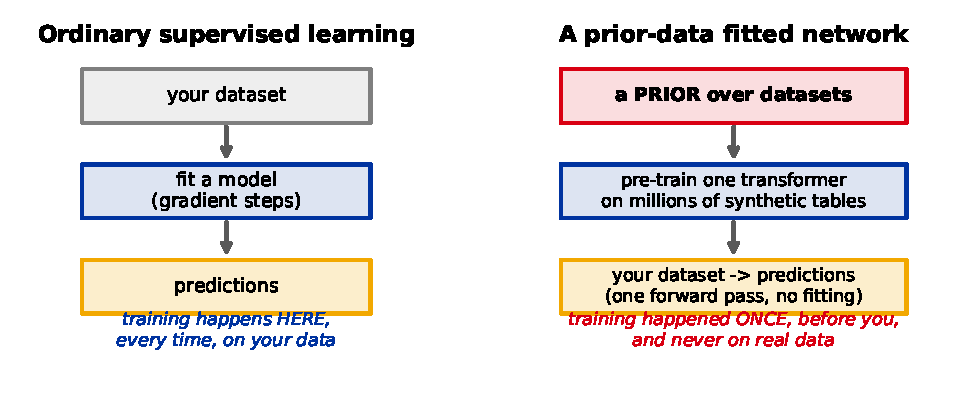
\includegraphics[width=0.86\textwidth]{pfn_inversion.pdf}
  \end{center}
  \vskip -2pt
  \footnotesize
  \centering
  The Nature paper's own phrase: \emph{"a learning algorithm that is itself learned across
  millions of synthetic datasets."}
\end{frame}

\begin{frame}{Say that sentence again, slowly}
  \small
  \emph{"A learning algorithm that is itself learned."} That sentence carries the whole
  lecture, and it is easy to nod at without it landing. So take it in two halves.
  \vskip 8pt
  \begin{columns}[T]
    \column{0.5\textwidth}
    \fcolorbox{armblue}{armblue!8}{\parbox{0.95\linewidth}{\footnotesize
      \textbf{What you have done until now.} You pick an algorithm - a tree, a linear model -
      and \emph{run} it on your data. The algorithm was written by a person. What comes out is
      a \textbf{fitted model}, $\fh$, and it is good for one dataset only.}}
    \column{0.5\textwidth}
    \fcolorbox{armred}{armred!8}{\parbox{0.95\linewidth}{\footnotesize
      \textbf{What happens here.} Somebody trained a network whose \emph{output behaviour} is
      the algorithm. It was never shown your data, or anybody's real data. Feed it a table and
      it behaves like a fitted model \textbf{without ever fitting}.}}
  \end{columns}
  \vskip 10pt
  \centering
  \fcolorbox{paramgreen}{paramgreen!8}{\parbox{0.94\linewidth}{\small\centering
    The thing that got \emph{learned} moved up one level: not the parameters of a model, but
    \textbf{the procedure that produces them}.}}
\end{frame}

\begin{frame}{The same weights, three different datasets}
  \small
  \begin{center}
    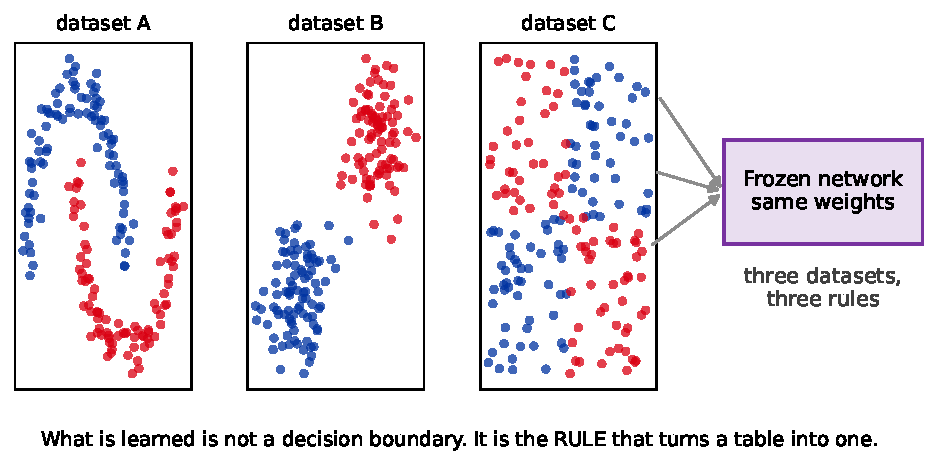
\includegraphics[width=0.72\textwidth]{one_model_many_datasets.pdf}
  \end{center}
  \vskip -4pt
  \fcolorbox{armblue}{armblue!8}{\parbox{0.97\linewidth}{\footnotesize
    A decision tree would need three training runs. Here \textbf{one frozen network} gives
    three different answers because each dataset supplies a different context.}}
\end{frame}

\begin{frame}{The recipe, in four steps}
  \small
  \begin{enumerate}\itemsep 5pt
    \item \textbf{Write down a prior} - an explicit generative process over datasets.
    \item \textbf{Sample millions of synthetic datasets} from it.
    \item \textbf{Train one transformer} to take $(\Xmat_{\text{train}}, \yv_{\text{train}},
      \Xmat_{\text{test}})$ and output a predictive distribution for $\yv_{\text{test}}$.
    \item \textbf{Ship it.} It is never trained again.
  \end{enumerate}
  \vskip 10pt
  \fcolorbox{armblue}{armblue!8}{\parbox{0.97\linewidth}{\small
    The object being learned is not a function $\fh$ for one dataset. It is
    \textbf{an algorithm} that maps any dataset to a prediction. Step 3 is the only training
    that ever happens, and it happens before you exist.}}
\end{frame}

\begin{frame}{At inference there is no fitting at all}
  \small
  You do not call \texttt{fit} in the usual sense. Labelled training rows provide the
  \textbf{context}; test rows have no labels. A base model predicts with \textbf{frozen
  weights}. Implementations may select rows, cache context or ensemble passes.
  \vskip 2pt
  \begin{center}
    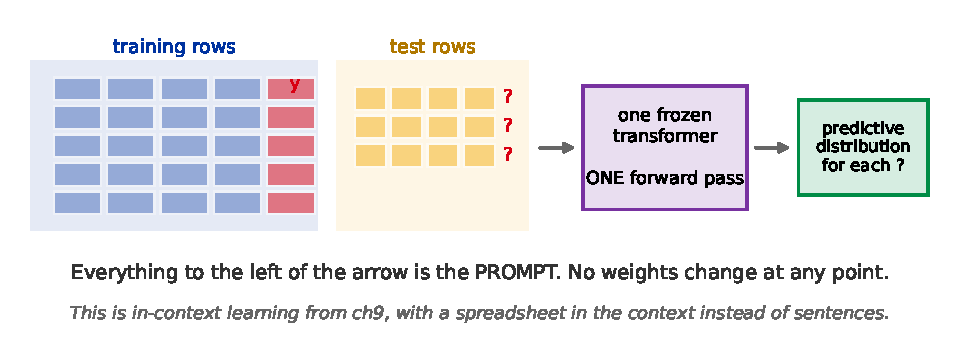
\includegraphics[width=0.94\textwidth]{incontext_layout.pdf}
  \end{center}
\end{frame}

\begin{frame}{What that changes for you}
  \small
  Nothing in that picture is a metaphor. There is genuinely no optimiser, no loop, and no
  fitted object at the end of it - which has consequences you will feel the first time you use
  the thing.
  \vskip 10pt
  \begin{columns}[T]
    \column{0.52\textwidth}
    \fcolorbox{paramgreen}{paramgreen!8}{\parbox{0.95\linewidth}{\footnotesize
      This is exactly \textbf{in-context learning}, which you met for language models - the same
      mechanism that lets an LLM pick up a pattern from examples in the prompt without any
      weight update. Here the "prompt" is a spreadsheet.}}
    \column{0.48\textwidth}
    \fcolorbox{armorange}{armorange!12}{\parbox{0.95\linewidth}{\footnotesize
      \textbf{Consequence:} there are no task-specific gradient steps, epochs or learning-rate
      schedule. Implementations can still preprocess and cache the training context, and can
      save a fitted estimator for reuse.}}
  \end{columns}
\end{frame}

\begin{frame}{Where does a synthetic dataset come from?}
  \small
  "Sampled from a prior over datasets" is the phrase that does all the work in this lecture, so
  here is that phrase performed once, end to end, on a table small enough to read.
  \vskip 2pt
  \begin{center}
    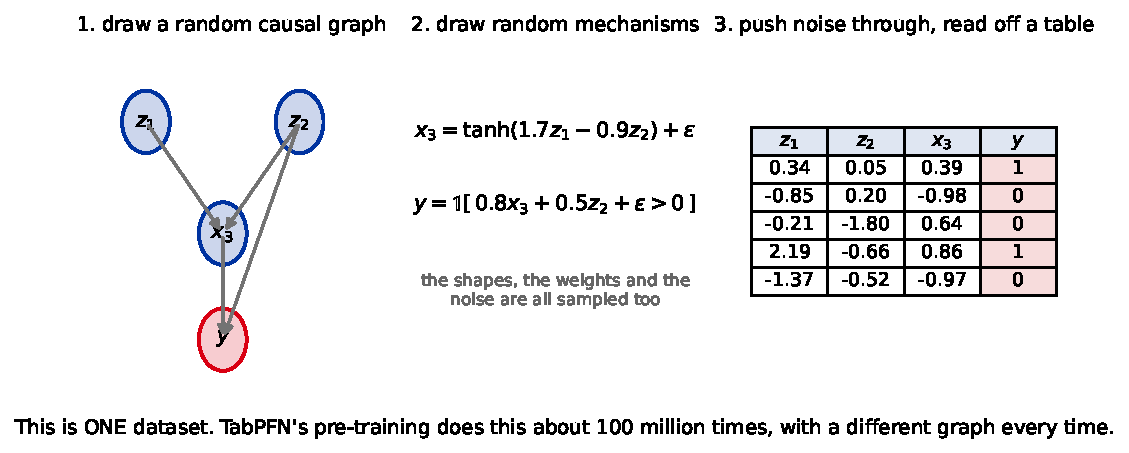
\includegraphics[width=0.95\textwidth]{scm_walkthrough.pdf}
  \end{center}
\end{frame}

\begin{frame}{A structural causal model: a table-making machine}
  \small
  A \textbf{structural causal model (SCM)} has three ingredients:
  \begin{enumerate}\itemsep 5pt
    \item A \textbf{directed graph}: arrows say which variables may directly affect which.
    \item One \textbf{equation per node}: a variable is computed from its parents.
    \item A fresh \textbf{noise draw per row}: otherwise every row would be identical.
  \end{enumerate}
  \vskip 7pt
  \begin{center}
    \fcolorbox{armblue}{armblue!8}{\parbox{0.91\linewidth}{\small\centering
      $z_1=\epsilon_1,\quad z_2=\epsilon_2,\quad
       x_3=\tanh(1.7z_1-0.9z_2)+\epsilon_3,\quad
       y=\mathbf{1}[0.8x_3+0.5z_2+\epsilon_y>0]$}}
  \end{center}
  \vskip 7pt
  Draw the graph and equations \emph{once}; draw new noise for each row. That gives one
  dataset. Draw a new graph, equations and noise to get the next dataset.
  \vskip 4pt
  \footnotesize
  These are \emph{synthetic causal stories}; the model is not discovering causal arrows in
  your real table. (Hollmann et al., 2025, Methods.)
\end{frame}

\begin{frame}{Where the Bayesian neural network enters}
  \small
  In a \textbf{Bayesian neural network (BNN)}, weights are uncertain: draw weights
  $\theta\sim p(\theta)$, then a function $f_\theta$ maps inputs to outputs.
  \vskip 5pt
  \begin{center}
    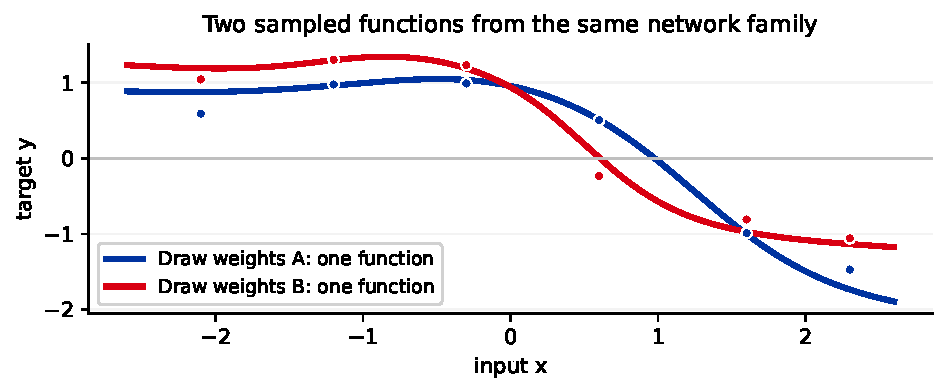
\includegraphics[width=0.74\textwidth]{bnn_prior.pdf}
  \end{center}
  \vskip -3pt
  \footnotesize
  \textbf{Two draws:} sampled weights choose a function for a \emph{dataset}; input and noise
  draws make its \emph{rows}. The original TabPFN mixed BNN and SCM generators
  (Hollmann et al., 2023). Nature v2 uses an SCM-based generator with neural mechanisms
  (Hollmann et al., 2025).
\end{frame}

\begin{frame}{Why that network is Bayesian}
  \small
  An ordinary trained neural network usually keeps one fitted weight vector
  $\hat\theta$. A BNN starts with a \textbf{distribution over weights} and updates that
  distribution after seeing labelled examples $D$:
  \vskip 8pt
  \begin{center}
    \fcolorbox{armblue}{armblue!8}{\parbox{0.9\linewidth}{\small\centering
      $p(\theta\mid D)\;\propto\;p(D\mid\theta)\,p(\theta)$
      \qquad and \qquad
      $p(y_*\mid x_*,D)=\int p(y_*\mid x_*,\theta)\,p(\theta\mid D)\,d\theta$}}
  \end{center}
  \vskip 8pt
  The prediction averages over plausible functions instead of betting on one set of weights.
  Exact integration is usually hard. A PFN is pre-trained on many draws from a prior so its
  forward pass \emph{approximates} a posterior predictive rule for new tasks.
  \vskip 4pt
  \footnotesize
  The PFN is not itself a BNN with weights updated on your table. The BNN is one possible
  \emph{generator of pre-training tasks}. (M\"uller et al., 2022; Hollmann et al., 2023.)
\end{frame}

\begin{frame}{A prior over datasets, not a prior over one answer}
  \small
  A single draw might yield a nearly linear table; another might yield thresholds,
  irrelevant columns or missing values. Pre-training repeatedly hides some labels and
  asks the transformer to predict them from the remaining rows.
  \vskip 8pt
  \begin{center}
    \fcolorbox{paramgreen}{paramgreen!8}{\parbox{0.92\linewidth}{\small\centering
      $\text{sample a data-making process}\;\longrightarrow\;
       \text{sample a table}\;\longrightarrow\;
       \text{hide labels}\;\longrightarrow\;
       \text{predict them}$}}
  \end{center}
  \vskip 8pt
  The PFN learns a predictor \emph{across tasks}. When your table arrives, its labels provide
  evidence about which synthetic patterns are useful. They do not update the network weights.
\end{frame}

\begin{frame}{Why invent the data at all?}
  \small
  It is a strange thing to do. Three reasons it is not a hack:
  \vskip 6pt
  \begin{columns}[T]
    \column{0.33\textwidth}
    \fcolorbox{armblue}{armblue!8}{\parbox{0.95\linewidth}{\footnotesize
      \textbf{You need millions.} There are not millions of clean, licensable real tables with
      the right shape. There are unlimited synthetic ones.}}
    \column{0.33\textwidth}
    \fcolorbox{paramgreen}{paramgreen!8}{\parbox{0.95\linewidth}{\footnotesize
      \textbf{You know the labels.} You generated the table, so you can hide labels and train
      directly on the prediction task. The PFN aims to approximate the posterior predictive
      answer for the prior.}}
    \column{0.33\textwidth}
    \fcolorbox{armorange}{armorange!12}{\parbox{0.95\linewidth}{\footnotesize
      \textbf{Less pre-training contamination.} The synthetic training corpus has no copied
      benchmark rows. Model selection and evaluation still need leakage checks.}}
  \end{columns}
  \vskip 10pt
  \centering
  \fcolorbox{armred}{armred!8}{\parbox{0.94\linewidth}{\footnotesize\centering
    And the bill: \textbf{patterns rare under the prior may be harder to predict.}
    Hold that thought - it connects to shift and benchmarking later.}}
\end{frame}

\begin{frame}{The prior, part 1: what is actually in it}
  \small
  Here are four draws from a small SCM generator. Each panel is a \emph{different task}:
  a new graph, new functions and new noise. Colors are generated labels.
  \vskip 2pt
  \begin{center}
    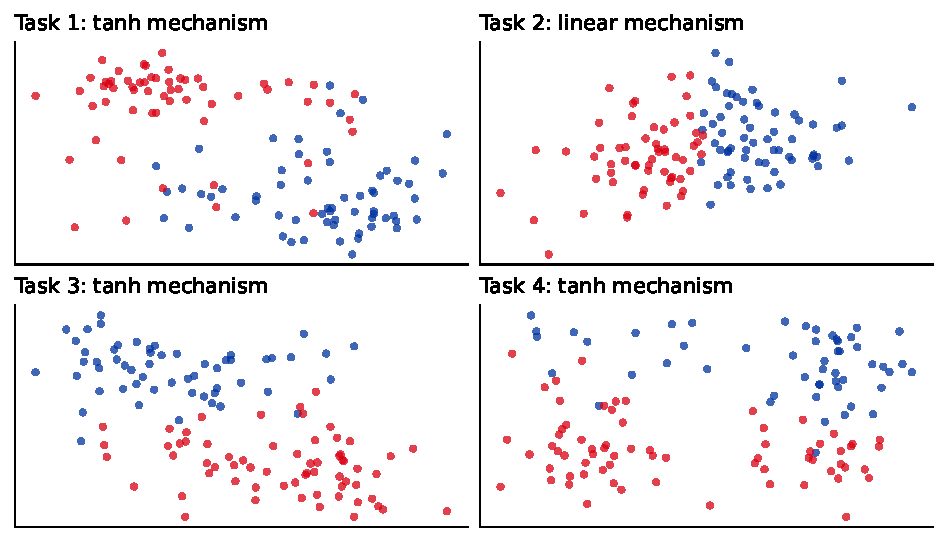
\includegraphics[width=0.77\textwidth]{prior_samples.pdf}
  \end{center}
  \vskip -3pt
  \footnotesize
  \centering
  Schematic draws generated for this slide, not samples from TabPFN's actual prior.
\end{frame}

\begin{frame}{The prior, part 2: the prior \emph{is} the inductive bias}
  \small
  This is the frame to hold on to. Everything later in the lecture is a consequence of it.
  \vskip 8pt
  \begin{columns}[T]
    \column{0.5\textwidth}
    \fcolorbox{armblue}{armblue!8}{\parbox{0.95\linewidth}{\footnotesize
      A tree's inductive bias is axis-aligned splits. A linear model's is additivity. A
      convolutional network's is locality.
      \vskip 3pt
      \textbf{A PFN's inductive bias is a probability distribution that somebody wrote down in
      code.}}}
    \column{0.5\textwidth}
    \footnotesize
    Three later frames are just this fact reappearing:
    \vskip 4pt
    \begin{itemize}\itemsep 2pt
      \item modelling shift can be helped by changing the prior;
      \item prior-induced bias can persist in some causal tasks;
      \item benchmarks resembling the prior may flatter the model.
    \end{itemize}
  \end{columns}
  \vskip 8pt
  \centering
  \footnotesize
  Change the prior and you have changed the model, without touching the architecture.
\end{frame}

\begin{frame}{"No training" is not "no cost"}
  \small
  A misconception worth killing early.
  \vskip 8pt
  \begin{columns}[T]
    \column{0.5\textwidth}
    \fcolorbox{armred}{armred!8}{\parbox{0.95\linewidth}{\small
      The pre-training \textbf{happened}. It was expensive. It ran once, on somebody else's
      hardware, on millions of generated datasets.}}
    \column{0.5\textwidth}
    \fcolorbox{paramgreen}{paramgreen!8}{\parbox{0.95\linewidth}{\small
      What changed is \textbf{who pays, and when}. The cost moved from your machine at your
      deadline to their machine, once, in advance.}}
  \end{columns}
  \vskip 10pt
  \centering
  \footnotesize
  That is the same trade as any pretrained model in this course - ch6's transfer learning, ch9's
  language models. The novelty is not free computation. It is that here the pre-training data
  was \textbf{invented} rather than collected.
\end{frame}

% ================================================================
\section{The architecture}

\begin{frame}[plain]
  \vfill
  \begin{center}
    {\Large\color{popblue}\textbf{The architecture}}\\[0.9em]
    \begin{minipage}{0.82\textwidth}\centering\small
      A table is not a sentence, and pretending otherwise is unaffordable.
    \end{minipage}
  \end{center}
  \vfill
\end{frame}

\begin{frame}{One representation per cell}
  \small
  The obvious thing is to flatten the table into a sequence of tokens and use an ordinary
  transformer. TabPFN does not. From the paper:
  \vskip 6pt
  \fcolorbox{armblue}{armblue!8}{\parbox{0.97\linewidth}{\footnotesize
    "an architecture that assigns a separate representation to \textbf{each cell} in the
    table\ldots{} a \textbf{two-way attention} mechanism, with each cell attending to the other
    features in its row (that is, its sample) and then attending to the same feature across its
    column (that is, all other samples)."}}
  \vskip 8pt
  So the state is indexed by \textbf{(row, column)}, not by position in a 1-D stream, and there
  are \textbf{two} distinct attention operations per layer rather than one.
\end{frame}

\begin{frame}{What attention computes for one cell}
  \small
  Every cell starts as a vector $h_{ij}$, where $i$ names a row and $j$ a feature.
  Attention replaces that vector with a learned \textbf{weighted mixture} of other vectors.
  \vskip 7pt
  \begin{center}
    \fcolorbox{armblue}{armblue!8}{\parbox{0.92\linewidth}{\small\centering
      $h^{\rm row}_{ij}=\sum_{k=1}^{m}a_{ijk}V(h_{ik})$
      \qquad then \qquad
      $h^{\rm col}_{ij}=\sum_{r=1}^{n}b_{ijr}V(h^{\rm row}_{rj})$}}
  \end{center}
  \vskip 7pt
  The weights $a$ and $b$ depend on the current cell and what it attends to.
  One layer therefore first combines features \emph{within a person}, then compares
  that result with the \emph{same feature across people}. Later layers repeat this.
  \vskip 5pt
  \footnotesize
  Diagram next: the highlighted cell is the query; orange cells are possible sources.
  (Hollmann et al., 2025, Methods.)
\end{frame}

\begin{frame}{What each direction is actually for}
  \small
  The two directions are not symmetric bookkeeping. They answer two different questions about
  one cell.
  \vskip 6pt
  \begin{columns}[T]
    \column{0.5\textwidth}
    \fcolorbox{armblue}{armblue!8}{\parbox{0.95\linewidth}{\footnotesize
      \textbf{Across the row: "who is this?"}\\[3pt]
      A salary of 3,000 means something different for a 20-year-old than for a 60-year-old.
      Row attention is how a cell sees the rest of \emph{its own sample}.}}
    \column{0.5\textwidth}
    \fcolorbox{paramgreen}{paramgreen!8}{\parbox{0.95\linewidth}{\footnotesize
      \textbf{Down the column: "is this big?"}\\[3pt]
      A raw number carries no scale. Column attention is how a cell sees \emph{the same feature
      in every other sample} - and so learns where it sits.}}
  \end{columns}
  \vskip 4pt
  \begin{center}
    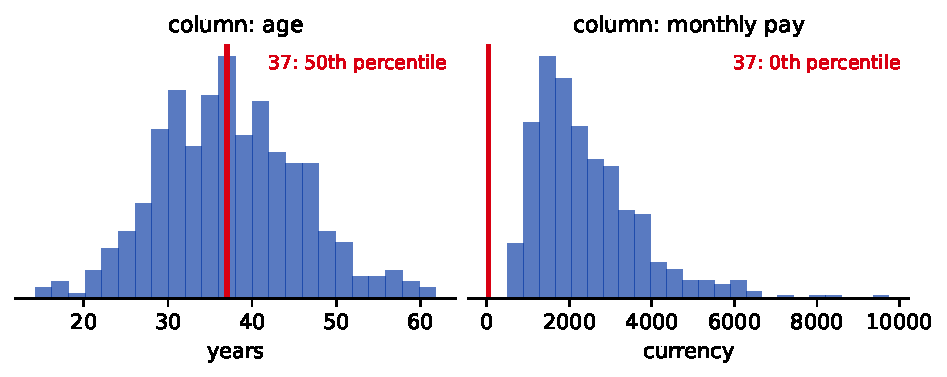
\includegraphics[width=0.82\textwidth]{column_meaning.pdf}
  \end{center}
\end{frame}

\begin{frame}{And that is why there is no scaler}
  \small
  In chapter 6 you standardised columns by hand. Here column attention can compare a value
  with other values in its feature; the implementation \emph{also} normalises numerical
  columns before the transformer.
  \vskip 8pt
  \fcolorbox{paramgreen}{paramgreen!8}{\parbox{0.97\linewidth}{\small
    The user usually need not run a separate scaler. The model's input pipeline handles
    normalisation, while attention can learn further comparisons within a column.}}
  \vskip 8pt
  \centering
  \footnotesize
  Do not claim attention alone makes scaling unnecessary. The Nature paper explicitly describes
  z-normalisation before the cell values are encoded (Hollmann et al., 2025, Methods).
\end{frame}

\begin{frame}{Two-way attention}
  \begin{center}
    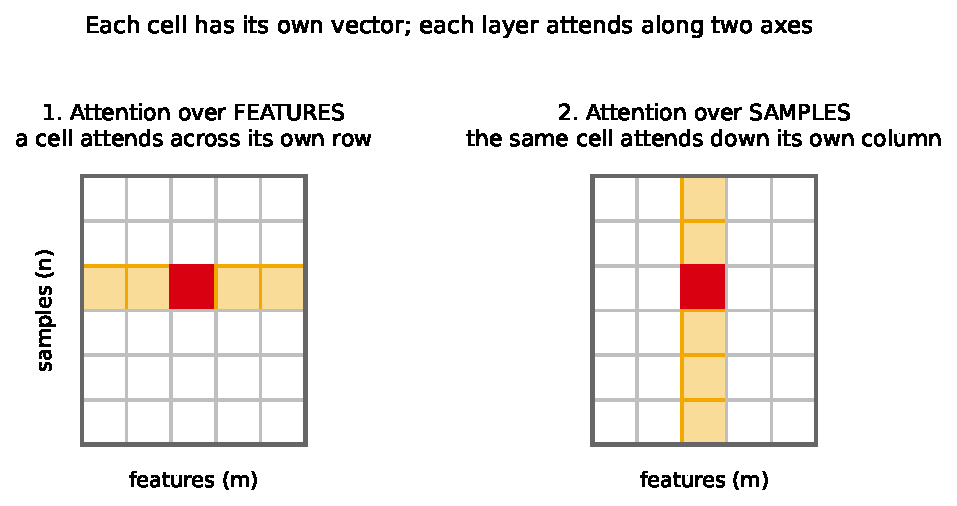
\includegraphics[width=0.84\textwidth]{two_d_attention.pdf}
  \end{center}
  \vskip -2pt
  \footnotesize
  \centering
  Then an MLP sublayer, with residual connections and normalisation, exactly as in ch9. Nothing
  about the transformer block itself is new here. What is new is \textbf{what attends to what}.
\end{frame}

\begin{frame}{Follow one prediction through both directions}
  \small
  Predict whether a patient has condition $y$ from age, blood pressure and a test result.
  \vskip 3pt
  \begin{center}
    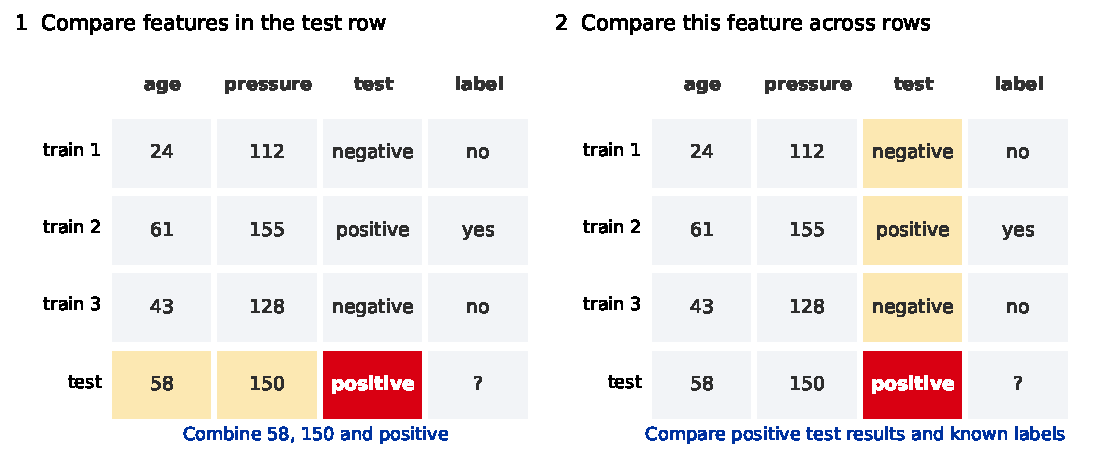
\includegraphics[width=0.94\textwidth]{attention_walkthrough.pdf}
  \end{center}
  \vskip -2pt
  \footnotesize
  Row attention can combine \emph{this patient's} measurements. Column attention can compare
  each transformed measurement with \emph{other patients}, including labelled examples.
  Test labels are masked; test rows cannot pass information to each other in the Nature model.
\end{frame}

\begin{frame}{Why this is different from other attention}
  \small
  \begin{tabular}{>{\raggedright\arraybackslash}p{2.15cm}>{\raggedright\arraybackslash}p{4.55cm}>{\raggedright\arraybackslash}p{4.7cm}}
    \toprule
    & \textbf{What can attend?} & \textbf{Order assumption} \\
    \midrule
    Text transformer & A token sees earlier tokens (or all tokens in an encoder). & Position matters: swapping words changes a sentence. \\
    Flat table transformer & Every one of $nm$ cell tokens can see every other cell. & Needs care to avoid inventing row/column order. \\
    TabPFN v2 & A cell sees its row, then its column; test labels stay hidden. & Row and feature permutations are built into the design. \\
    \bottomrule
  \end{tabular}
  \vskip 7pt
  \footnotesize
  "Two-way" means \textbf{two axes of a table}, not bidirectional language attention.
  The effective context is still the labelled training set.
\end{frame}

\begin{frame}{Predict first}
  \small
  Take your test table and \textbf{permute the columns} - same data, different order. Then
  permute the rows.
  \vskip 10pt
  \begin{center}
    \textbf{Do the predictions change?}
  \end{center}
  \vskip 10pt
  \pause
  \begin{columns}[T]
    \column{0.5\textwidth}
    \fcolorbox{paramgreen}{paramgreen!8}{\parbox{0.95\linewidth}{\small
      \textbf{No.} And not because the model learned not to care. The paper: this design
      \textbf{"enables the architecture to be invariant to the order of both samples and
      features."}}}
    \column{0.5\textwidth}
    \fcolorbox{armblue}{armblue!8}{\parbox{0.95\linewidth}{\small
      \textbf{The invariance is architectural.} Same idea as a convolutional network's
      translation equivariance in ch6 - build the symmetry into the wiring instead of hoping
      data teaches it.}}
  \end{columns}
  \vskip 8pt
  \centering
  \footnotesize
  A row-order-dependent model would be absurd for a spreadsheet. A sequence model would have to
  learn its way out of that. This one cannot express it in the first place.
\end{frame}

\begin{frame}{Worked numbers: why the factorisation matters}
  \small
  Suppose $n$ rows and $m$ features, so $n \cdot m$ cells.
  \vskip 4pt
  \begin{columns}[T]
    \column{0.5\textwidth}
    \footnotesize
    \textbf{Naive:} one sequence of all $n\cdot m$ cells. Attention is quadratic in sequence
    length, so $(n \cdot m)^2$ pairs.
    \vskip 5pt
    \textbf{Two-way:} $n$ row attentions of length $m$, then $m$ column attentions of length $n$:
    $$n m^2 + m n^2 = nm(n+m) \text{ attention pairs.}$$
    The Nature paper summarises the separate quadratic dependence on $n$ and $m$ as
    $O(n^2+m^2)$ when describing scaling along either axis.
    \column{0.5\textwidth}
    \vskip 2pt
    \footnotesize
    At $n = 10{,}000$ and $m = 100$:
    \vskip 3pt
    \begin{center}
      \begin{tabular}{lr}
        \toprule
        naive & $10^{12}$ \\
        two-way & $1.01\times10^{10}$ \\
        \midrule
        \textbf{ratio} & $\mathbf{\approx 99\times}$ \\
        \bottomrule
      \end{tabular}
    \end{center}
    \vskip 4pt
    \fcolorbox{paramgreen}{paramgreen!8}{\parbox{0.95\linewidth}{\scriptsize
      These are counts of possible attention pairs, not wall-clock speed or GPU memory.
      Optimised inference and caching matter too.}}
  \end{columns}
\end{frame}

\begin{frame}{The cost, plotted}
  \begin{center}
    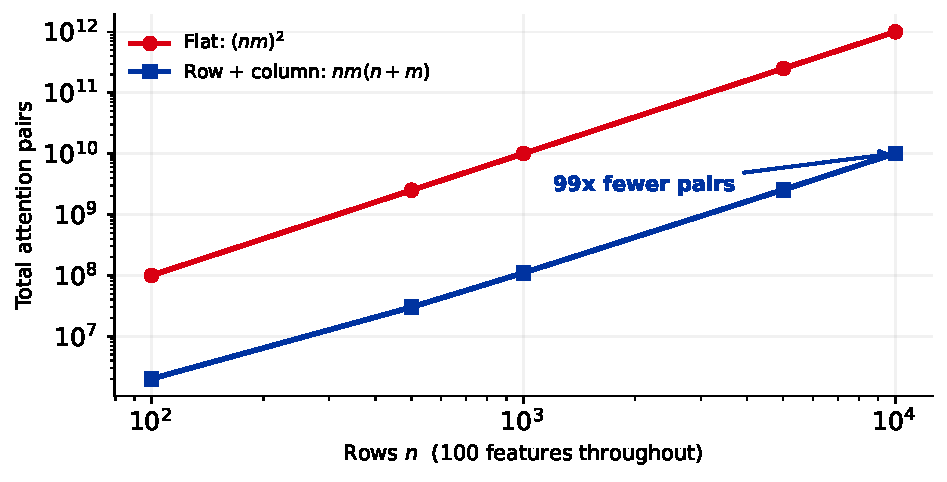
\includegraphics[width=0.79\textwidth]{context_cost.pdf}
  \end{center}
  \vskip -2pt
  \footnotesize
  \centering
  The paper reports optimised inference memory scaling with $nm$, under 1,000 bytes per cell.
  Its 10,000-row result is an \emph{accuracy benchmark boundary}, not a hard context limit.
\end{frame}

% ================================================================
\section{The landscape}

\begin{frame}[plain]
  \vfill
  \begin{center}
    {\Large\color{popblue}\textbf{The landscape}}\\[0.9em]
    \begin{minipage}{0.82\textwidth}\centering\small
      One idea, several models, and a licence you should read.
    \end{minipage}
  \end{center}
  \vfill
\end{frame}

\begin{frame}{The TabPFN line}
  \small
  \begin{center}
    \footnotesize
    \begin{tabular}{ll>{\raggedright\arraybackslash}p{5.4cm}}
      \toprule
      \textbf{When} & \textbf{What} & \textbf{Rows it claims to handle} \\
      \midrule
      2021 & Transformers Can Do Bayesian Inference & the founding idea, before tables \\
      2022 & TabPFN v1 & pre-trained on sizes up to about 1,000 \\
      \rowcolor{armred!12}
      2025 & \textbf{TabPFN v2} (Nature) & \textbf{wins up to 10,000} - peer reviewed \\
      2025 & TabPFN-2.5 & 50,000 x 2,000 \\
      2026 & TabPFN-3 & up to \textbf{1,000,000} x 200 - vendor benchmark \\
      2026 & TabPFN-3.5 (current default) & up to 1M rows x 20k features - recommended limit \\
      \bottomrule
    \end{tabular}
  \end{center}
  \vskip 4pt
  \footnotesize
  \textbf{Do not read the last column as one benchmark.} Nature v2's 10,000 is a
  peer-reviewed accuracy claim; later numbers mix vendor benchmarks and supported sizes.
  The default and limits were checked in the Prior Labs documentation, October 2026.
\end{frame}

\begin{frame}{The neighbours}
  \small
  TabPFN is not the only table foundation model. Alternatives differ in where
  pre-training data comes from and how many rows they handle.
  \vskip 9pt
  \footnotesize
  \begin{itemize}\itemsep 8pt
    \item \textbf{TabICL} (Tabular In-Context Learning) and TabICLv2 - built for larger tables,
      and open.
    \item \textbf{TabDPT} - pre-trains on \textbf{real} data instead of a purely synthetic prior.
    \item \textbf{LimiX} - a further entrant, 2026.
  \end{itemize}
  \vskip 6pt
  The idea also extends to time-series forecasting, relational tables and mixed modalities.
  These extensions often use different checkpoints or pipelines.
\end{frame}

\begin{frame}{What prediction task are you asking it to solve?}
  \small
  The standard interface is \textbf{supervised prediction}: each training row has features
  and a target; the model predicts targets for new rows.
  \vskip 6pt
  \begin{tabular}{>{\raggedright\arraybackslash}p{3.2cm}>{\raggedright\arraybackslash}p{4.2cm}>{\raggedright\arraybackslash}p{4.0cm}}
    \toprule
    \textbf{Target} & \textbf{Example} & \textbf{Interface} \\
    \midrule
    Binary class & fraud / no fraud & classifier, probabilities \\
    Multiple classes & one of several diagnoses & classifier, class probabilities \\
    Continuous value & house price & regressor, value or distribution \\
    \bottomrule
  \end{tabular}
  \vskip 8pt
  \fcolorbox{armorange}{armorange!12}{\parbox{0.94\linewidth}{\footnotesize
    v1 was classification only. The Nature v2 paper added regression. Time-series,
    relational and text-heavy tasks use later checkpoints or specialised workflows;
    they are not implied by the simple classifier call.}}
\end{frame}

\begin{frame}{Can I give it categorical, missing or text fields?}
  \footnotesize
  \begin{tabular}{>{\raggedright\arraybackslash}p{2.0cm}>{\raggedright\arraybackslash}p{4.45cm}>{\raggedright\arraybackslash}p{4.8cm}}
    \toprule
    \textbf{Input} & \textbf{Practical answer} & \textbf{Boundary} \\
    \midrule
    Numbers & Yes: ages, prices, counts. & Usually leave scaling to the pipeline. \\
    Categories & Yes in v2 and later: e.g. city, plan type. & Preserve category meaning; do not treat codes as ordered numbers. \\
    Missing cells & Yes in v2 and later. & Investigate the missingness mechanism; support is not a guarantee of accuracy. \\
    Free text & For meaning, use text embeddings or a text-capable 3.5 workflow. & Base 3.5 benchmark encodes strings; Plus/Thinking process raw text directly. \\
    Images & Use an image encoder or a multimodal workflow. & A path or raw pixel array is not a semantic tabular feature. \\
    Dates & Use valid datetime input or derived time features. & A date-looking string may be treated as text/category. \\
    \bottomrule
  \end{tabular}
  \vskip 5pt
  \scriptsize
  Sources: Hollmann et al. (2025); J\"ager et al., TabPFN-3.5 report (2026);
  Prior Labs current documentation. Check the exact checkpoint and API before teaching a demo.
\end{frame}

\begin{frame}{What the simple table interface does not solve for you}
  \small
  \begin{itemize}\itemsep 6pt
    \item \textbf{Evaluation design:} split by time or group when deployment will; random row
      splits can flatter any model.
    \item \textbf{Information missing from the table:} joins and domain features still matter.
    \item \textbf{Scale and hardware:} recommended row/feature limits depend on checkpoint;
      a GPU is strongly preferred for large tables.
    \item \textbf{Target structure:} ordinary classification/regression is the core API.
      Forecasting, relational prediction and other tasks need specialised pipelines.
    \item \textbf{Use rights:} code and model weights have separate licences.
  \end{itemize}
  \vskip 4pt
  \footnotesize
  A useful default is to benchmark TabPFN against a tuned tree model on \emph{your}
  validation split and check memory, latency and licence for the chosen checkpoint.
\end{frame}

\begin{frame}{Using it}
  \small
  The current default interface (TabPFN-3.5). The 2.8-second comparison earlier in the
  deck was for \emph{TabPFN v2}, not this checkpoint.
  \vskip 8pt
  \begin{center}
    \fcolorbox{lightbg}{lightbg}{\parbox{0.86\linewidth}{\ttfamily\small
      from tabpfn import TabPFNClassifier \\[3pt]
      clf = TabPFNClassifier() \\
      clf.fit(X\_train, y\_train) \\
      y\_pred = clf.predict(X\_test)
    }}
  \end{center}
  \vskip 8pt
  \fcolorbox{armorange}{armorange!12}{\parbox{0.97\linewidth}{\footnotesize
    \texttt{fit} does \textbf{not update the foundation model's weights}. It validates and
    preprocesses data and may prepare or cache the training context. \texttt{predict} uses
    that context to answer new rows. The first run may download weights.}}
\end{frame}

% ================================================================
\section{What is it actually doing?}

\begin{frame}[plain]
  \vfill
  \begin{center}
    {\Large\color{popblue}\textbf{What is it actually doing?}}\\[0.9em]
    \begin{minipage}{0.82\textwidth}\centering\small
      Nobody agrees, including the people who built it.
    \end{minipage}
  \end{center}
  \vfill
\end{frame}

\begin{frame}{Why does it improve on tables bigger than anything it pre-trained on?}
  \small
  That question has no agreed answer, and the disagreement is in print.
  \vskip 6pt
  \begin{columns}[T]
    \column{0.48\textwidth}
    \fcolorbox{armblue}{armblue!8}{\parbox{0.95\linewidth}{\footnotesize
      \textbf{The Bayesian reading.} The network approximates the \textbf{posterior predictive}
      under the prior. Generalisation in context is Bayesian updating.
      \vskip 3pt
      \emph{Müller, Hollmann \& Hutter (2024)} - the TabPFN authors.}}
    \column{0.48\textwidth}
    \fcolorbox{armred}{armred!8}{\parbox{0.95\linewidth}{\footnotesize
      \textbf{The frequentist reading.} A PFN is a \textbf{pre-tuned but untrained} predictor.
      No posterior needed - and this version explains improvement on tables larger than any seen
      in pre-training.
      \vskip 3pt
      \emph{Nagler (ICML 2023)}.}}
  \end{columns}
  \vskip 8pt
  \fcolorbox{armorange}{armorange!12}{\parbox{0.97\linewidth}{\footnotesize
    And a third result unsettles both. Estimating a treatment effect, PFNs \emph{can} exhibit
    \textbf{prior-induced confounding bias: "the prior is not asymptotically overwritten by
    data"} (Melnychuk et al., 2026), which breaks frequentist consistency - the property you
    were taught to expect from an estimator. The same paper gives a correction that restores it.
    The lesson is not that the model is broken; it is that, as two frames ago, \textbf{the prior
    is the model}.}}
\end{frame}

% ================================================================
\section{Where it stops winning}

\begin{frame}[plain]
  \vfill
  \begin{center}
    {\Large\color{popblue}\textbf{Where it stops winning}}\\[0.9em]
    \begin{minipage}{0.82\textwidth}\centering\small
      The honest half. It is most of the lecture's value.
    \end{minipage}
  \end{center}
  \vfill
\end{frame}

\begin{frame}{Papers that extend the context}
  \begin{center}
    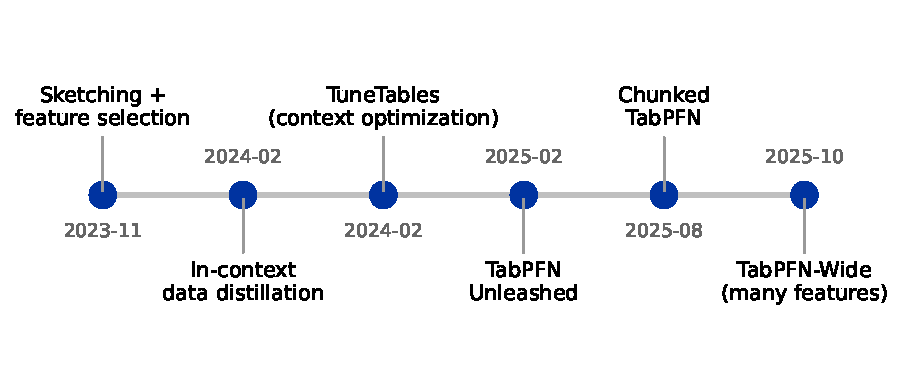
\includegraphics[width=0.86\textwidth]{scaling_timeline.pdf}
  \end{center}
  \vskip -4pt
  \footnotesize
  The methods select or distil rows, chunk long contexts, or handle many features.
  Table size is a real \textbf{computational constraint}.
  \vskip 3pt
  \fcolorbox{armorange}{armorange!12}{\parbox{0.97\linewidth}{\footnotesize
    \textbf{The boundary moved.} Nature v2 won up to 10,000 rows (2025); the vendor reports
    one million for TabPFN-3 (2026). Compare on your own validation split.}}
\end{frame}

\begin{frame}{Distribution shift needed its own model}
  \small
  Real tables drift. Prices change, populations change, the sensor gets recalibrated.
  \vskip 8pt
  \begin{columns}[T]
    \column{0.5\textwidth}
    \fcolorbox{armblue}{armblue!8}{\parbox{0.95\linewidth}{\footnotesize
      \textbf{Drift-Resilient TabPFN} (2024) handles temporal shift by putting shift
      \textbf{into the prior}: pre-train on synthetic datasets that already drift.}}
    \column{0.5\textwidth}
    \fcolorbox{armred}{armred!8}{\parbox{0.95\linewidth}{\footnotesize
      This shows why the \textbf{evaluation split matters}. The Nature v2 benchmark does not
      establish robustness to future distribution shift. Later models improve this, but
      check on the shift you expect.}}
  \end{columns}
  \vskip 10pt
  \centering
  \footnotesize
  The prior can be changed to include shift, and newer training recipes can help; neither
  removes the need for a time-aware test on your problem.
\end{frame}

\begin{frame}{The benchmark problem}
  \small
  A model pre-trained on a prior over structural causal models will do well on benchmark
  datasets that \textbf{look like draws from that prior}.
  \vskip 8pt
  \begin{columns}[T]
    \column{0.52\textwidth}
    \footnotesize
    \emph{Realistic Evaluation of TabPFN v2 in Open Environments} (2025) asks what happens when
    the quiet assumptions of a benchmark suite stop holding - clean features, no shift, a closed
    label set.
    \vskip 5pt
    That is not a criticism unique to this model. It is the question you should ask of any
    reported win.
    \column{0.48\textwidth}
    \fcolorbox{armorange}{armorange!12}{\parbox{0.95\linewidth}{\footnotesize
      You have the tools for this already. This is
      \texttt{27\_stat\_how\_to\_lie} applied to a \textbf{benchmark culture} rather than to a
      single experiment.}}
  \end{columns}
  \vskip 8pt
  \fcolorbox{armred}{armred!8}{\parbox{0.97\linewidth}{\footnotesize
    \textbf{Apply it to this lecture.} The 10,000-row figure is from a \textbf{peer-reviewed
    Nature paper}. The 1,000,000-row figure is from the \textbf{vendor, on its own benchmarks}.
    Both may well be right. They are not the same kind of evidence, and a slide that printed
    them in the same font would be misleading you.}}
\end{frame}

\begin{frame}{Feature engineering: chapter 6 already measured this}
  \small
  A tempting overclaim is that this kills feature engineering. Chapter 6 got there first, with
  numbers, and was more careful:
  \vskip 6pt
  \begin{center}
    \fcolorbox{armblue}{armblue!8}{\parbox{0.9\linewidth}{\centering\small
      Feature engineering was worth \textbf{$+81.5$ MAE to Ridge} and \textbf{$-4.3$ to a
      forest.}\\
      \emph{"Feature engineering is not dead - it moved."}}}
  \end{center}
  \vskip 8pt
  \footnotesize
  A capable model already absorbed most of what feature engineering used to buy - ch6 measured
  it \emph{hurting} the forest. A tabular foundation model pushes further in the same direction.
  \vskip 5pt
  It does not touch the part ch6 said still pays: \textbf{joins, domain knowledge, and the
  features no model can derive because the information is not in the table.} Research in 2026
  (\emph{TabPrep}) is actively arguing the gap is still there.
\end{frame}

\begin{frame}{The licence}
  \small
  This one changes what you are allowed to build, so it is not a footnote.
  \vskip 6pt
  \fcolorbox{armred}{armred!8}{\parbox{0.97\linewidth}{\small
    The \textbf{model weights} (2.5, 2.6, 3 and 3.5) are released under \textbf{non-commercial}
    licences: research and internal evaluation are fine, commercial and production use are
    \textbf{not} - explicitly including the model's \textbf{outputs}.
    \vskip 3pt
    The \textbf{code} is separate and permissive (Apache 2.0 with an attribution requirement).
    \textbf{Free code, restricted weights} is a pattern you will meet again.}}
  \vskip 8pt
  \begin{columns}[T]
    \column{0.5\textwidth}
    \footnotesize
    "Outputs" is broad. Generating a feature with it, or labelling data with it, produces a
    covered output.
    \column{0.5\textwidth}
    \fcolorbox{paramgreen}{paramgreen!8}{\parbox{0.95\linewidth}{\footnotesize
      Which makes \textbf{TabICLv2} being open a real engineering decision, not a footnote:
      slightly different model, entirely different set of things you may ship.}}
  \end{columns}
  \vskip 8pt
  \centering
  \footnotesize
  "Beats gradient boosting" and "cannot go in your product" belong on the same slide.
\end{frame}

% ================================================================
\section*{Wrap-up}

\begin{frame}{Recap}
  \small
  \begin{columns}[T]
    \column{0.54\textwidth}
    \begin{enumerate}\footnotesize\itemsep 3pt
      \item A prior-data fitted network is trained on a \textbf{prior over datasets}, not on
        your dataset. Your table is context, not training data.
      \item \textbf{The prior is an inductive bias.} Shift and benchmark design matter;
        some causal estimands can retain prior-induced bias.
      \item Two-way attention gives \textbf{order invariance by construction}; counting all
        attention pairs gives $nm(n+m)$ instead of $(nm)^2$ - about $99\times$ fewer at
        $n{=}10{,}000$, $m{=}100$.
      \item The Nature v2 model beat four hours of tuning in 2.8 seconds on its benchmark;
        newer versions handle larger tables and more input types.
      \item Nobody agrees on what it is doing, including its authors.
    \end{enumerate}
    \column{0.46\textwidth}
    \vskip 10pt
    \fcolorbox{paramgreen}{paramgreen!8}{\parbox{0.95\linewidth}{\small
      \textbf{What to do with this.}
      \vskip 4pt
      On a small clean table, \textbf{try the forward pass first}. It costs seconds, and
      chapter 4's four hours of tuning is what you are saving.
      \vskip 4pt
      Compare with tuned boosting on your own split, especially under shift, with messy
      data or with deployment constraints.
      \vskip 4pt
      \textbf{Do not memorise a row threshold.} Look up the current one - it has moved every
      year so far.}}
    \vskip 5pt
    \fcolorbox{armblue}{armblue!8}{\parbox{0.95\linewidth}{\footnotesize
      The transferable idea: \textbf{if you can write down where your problems come from, you
      can learn the algorithm instead of the answer.}}}
  \end{columns}
\end{frame}

\end{document}

% ================================================================
% Provenance:
%   Deck: L37 Tabular Foundation Models. Original 2026-08-08; revised 2026-10-14.
%   Primary papers: Hollmann et al. (ICLR 2023, arXiv:2207.01848),
%     Hollmann et al. (Nature 2025, DOI:10.1038/s41586-024-08328-6),
%     Prior Labs TabPFN-3 report (arXiv:2605.13986), and Jager et al.
%     TabPFN-3.5 report (arXiv:2609.17895). PDFs in papers/.
%   Current model/API/licence details: github.com/PriorLabs/TabPFN,
%     checked 2026-10-14. Version-specific limits may change.
%   Figures: py_src/l37_tabular_figs.py -> fig/. Illustrative synthetic
%     plots and diagrams, never measured TabPFN outputs.
%   Revision: expands SCMs and BNNs; works through axial attention;
%     distinguishes basic tasks and input types across versions; updates 3.5;
%     corrects attention-pair arithmetic to nm(n+m), not n^2+m^2 total.
%   The Nature paper describes scaling as O(n^2+m^2) along the two axes;
%     the per-row and per-column counts across the full table retain
%     multiplicities n and m. At n=10,000,m=100, 10^12/1.01e10 ~ 99.
